% !TeX root = ../main.tex

\paragraph{Homework \#1 Free electron model}

\begin{problem}[Two-charge-carrier Drude model]
  Consider a system of two types of charge carriers in the Drude model.
  The two carriers have the same density ($n$)
  and opposite charge ($e$ and $-e$),
  and their massesand relaxation rates are $m_1$, $m_2$ and $\tau_1$, $\tau_2$,
  respectively.
  So their corresponding mobilities are $\mu_1 = \frac{e\tau_1}{m_1}$ and
  $\mu_2 = \frac{e\tau_2}{m_2}$, respectively.
  \begin{enumext}[label = (\alph*)]
    \item Calculate the magnetoresistance $\Delta \rho = \rho(B) - \rho(B = 0)$,
    where $B$ is the magnetic field.
    \item Calculate the Hall coefficient.
    \item In an undoped semiconductor, $n = n_0 \upe^{-\Delta/k_BT}$
    describes the temperature dependence of the carrier concentration.
    What will the temperature dependence of the magnetoresistance
    and the Hall coefficient be?
  \end{enumext}
\end{problem}
\begin{solution}\leavevmode
  \begin{enumext*}[label = (\alph*), columns = 2]
    \item(2) Assume $\bm B = (0,0,B)$. Then, the resistance tensor
    \begin{gather*}
        \hat\rho = \hat\sigma^{-1}
      = \frac{1}{\sigma_{xx}^2 + \sigma_{xy}^2}
      \begin{psmallmatrix}
        \sigma_{xx} & -\sigma_{xy} & 0\\
        \sigma_{xy} & \sigma_{xx}  & 0\\
        0 & 0 & (\sigma_{xx}^2+\sigma_{xy}^2)/\sigma_{zz}
      \end{psmallmatrix}\\
      \begin{array}{@{}l@{~}c@{~}l@{\quad}l@{~}c@{~}l@{}}
        \sigma_{xx} & = & \sigma_{yy}
      = \frac{\sigma_0}{1 + \omega_{c_i}^2\tau_i^2}, &
        \sigma_{xy} & = & -\sigma_{yx}
      = \frac{\sigma_0\omega_{c_i}\tau_i}{1 + \omega_{c_i}^2\tau_i^2},\\
        \sigma_{zz} & = & \sigma_0 = nq^2\tau_i/m_i, &
        \omega_c    & = & Bq/m_i,
      \end{array}
    \end{gather*}
    For double charge carriers,
    $\sigma_{ij}^\text{tot} = \sigma_{ij}^{(1)} + \sigma_{ij}^{(2)}$.
    Then
    \[
      \rho_{xx} = \frac{1 + B^2\mu_1 \mu_2}{ne(\mu_1 + \mu_2)}, \quad
      \rho_{xy} = \frac{B(\mu_2 - \mu_1)}{ne(\mu_1 + \mu_2)}
    \]
    and the differences
    \[
      \Delta\rho_{xx} = \frac{B^2\mu_1\mu_2}{ne(\mu_1 + \mu_2)},\quad
      \Delta\rho_{xy} = \frac{B(\mu_1 - \mu_2)}{ne(\mu_1 + \mu_2)}.
    \]
    \item $R_H = \frac{\rho_{xy}}B = \frac{\mu_2 - \mu_1}{ne(\mu_1 + \mu_2)}$.
    \item $R_H$, $\Delta \rho \propto \upe^{\Delta/k_BT}$.
  \end{enumext*}
\end{solution}

\begin{wrapstuff}[width = .32\linewidth, lines = 6]
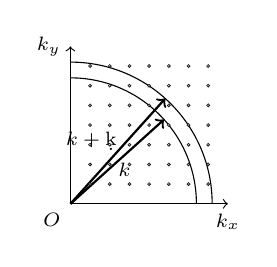
\begin{tikzpicture}[scale = .5, font = \scriptsize]
  \draw [<->] (0,4) node [left] {$k_y$} -- (0,0)
                    node [below left] {$O$} -- (4,0) node [below] {$k_x$};
  \draw (3.2,0) arc (0:90:3.2) (3.6,0) arc (0:90:3.6);
  \draw [thick, ->] (0,0) -- node [inner sep = 0pt, below right]
    {$k$} (42:3.2);
  \draw [thick, ->] (0,0) -- node [inner sep = 0pt, above left]
    {$k + \d k$} (48:3.6);
  \foreach \j in {1, ..., 7} \foreach \i in {1, ..., 7}
    \shade [shift = {(.5*\i, .5*\j)}, ball color = black]
      (0,0) circle (.05);
\end{tikzpicture}
\end{wrapstuff}
\begin{problem}[Density of States in 2D system]
  Consider free electron in a 2D box with a width of $a$.
  The allowed wave-numbers $k_x$ and $k_y$ for $x$ and $y$ directions
  respectively are expressed as $\frac{\pi n_x}a$ and $\frac{\pi n_y}{a}$,
  where $n_x$, $n_y = 1$, $2$, $3$, $\ldots$ are integer numbers.
  The following figure shows the schematic view of the 2D array of
  allowed quantum states in $k$-space.
  \wrapstuffclear
  \begin{enumext}[label = (\alph*)]
    \item Determine the area in $k$-space occupied by 1 allowed $k$ point.
    \item Express number of allowed states in the area enclosed
    by the first quarter circles with the radus of $k$ and $k + \d k$,
    where $k \gg \d k$ (Consider the spin degeneracy).
    \item Express density of allowed states in real space per unit energy.
  \end{enumext}
\end{problem}
\begin{solution}\leavevmode
  \begin{enumext}[label = (\alph*)]
    \item The area is
    $\Delta\bm k = \Delta k_x \cdot \Delta k_y = \ab(\frac\pi a)^2$.
    \item Two electrons can occupy each site
    \[
      \d N = 2 \times \frac{\d A}{\Delta \bm k}
    = \frac{\frac14[\pi(k + \Delta k)^2 - \pi k^2]}{(\pi/a)^2}
    \approx \frac{a^2k}{\pi}\d k.
    \]
    with $\ket|\uparrow>$ and $\ket|\downarrow>$.
    \item Substituting into the definition of DOS
    \[
      \text{DOS} = \frac{\d N}{\Delta A \d E}
      \xlongequal{E = \hbar^2k^2/2m} \frac{\odv N/k}{\Delta A \odv E/k}
    = \frac{m}{\pi \hbar^2}.
    \]
  \end{enumext}
\end{solution}

\begin{problem}[Density of states from a general formula]\leavevmode
  \begin{enumext}[label = (\alph*)]
    \item In a 3D solid and starting from the general formula
    \[
      g(E) = \frac{2V}{(2\pi)^3} \iint \frac{\d S_E}{|\nabla_kE|}.
    \]
    Find the expression for the electronic density of states:
    \begin{enumerate*}[label = (\roman*)]
      \item for free electrons;
      \item for electrons that obey the isotropic dispersion relation:
      $E = -E_0 - 2\gamma \cos\ab(\frac{ka}{2})$, where $E_0$, $\gamma > 0$.
    \end{enumerate*}
    \item After having established the corresponding expression for 2D,
    find $g(E)$ for (i) and (ii) above.
    \item Same question for 1D.
  \end{enumext}
\end{problem}
\begin{solution}
  In 3D, 2D, and 1D situations, the DOS are
  \begin{align*}
    g_\text{3D}(E) & = \frac{2V}{(2\pi)^3} \cdot \frac{4\pi k^2}{\nabla_kE}
  = \begin{cases}
      \frac{mV}{\pi^2\hbar^3}\sqrt{2mE},\\
      \frac{8V}{\pi^2a^3} \frac{\ab[\arccos\ab(\frac{E + E_0}{2\gamma})]}
        {\sqrt{4\gamma^2 - (E + E_0)^2}}.
    \end{cases}\\
    g_\text{2D}(E) & = \frac{2A}{(2\pi)^2} \cdot \frac{2\pi k}{\nabla_kE}
  = \begin{cases}
      \frac{mA}{\pi\hbar^2} = \text{Const},\\
      \frac{4A}{\pi a^2} \frac{\arccos\ab(-\frac{E+E_0}{2\gamma})}
        {\sqrt{4\gamma^2 - \ab(E + E_0)^2}}.
    \end{cases}\\
    g_\text{1D}(E) & = \frac{2L}{2\pi} \cdot \frac{2}{\odv E/k}
  = \begin{cases}
      \frac L{\pi\hbar} \sqrt{\frac{2m}{E}},\\
      \frac{4L}{\pi a} \frac{1}{\sqrt{4\gamma^2 - \ab(E + E_0)^2}}.
    \end{cases}
  \end{align*}
\end{solution}